\hypertarget{page1-div}{}
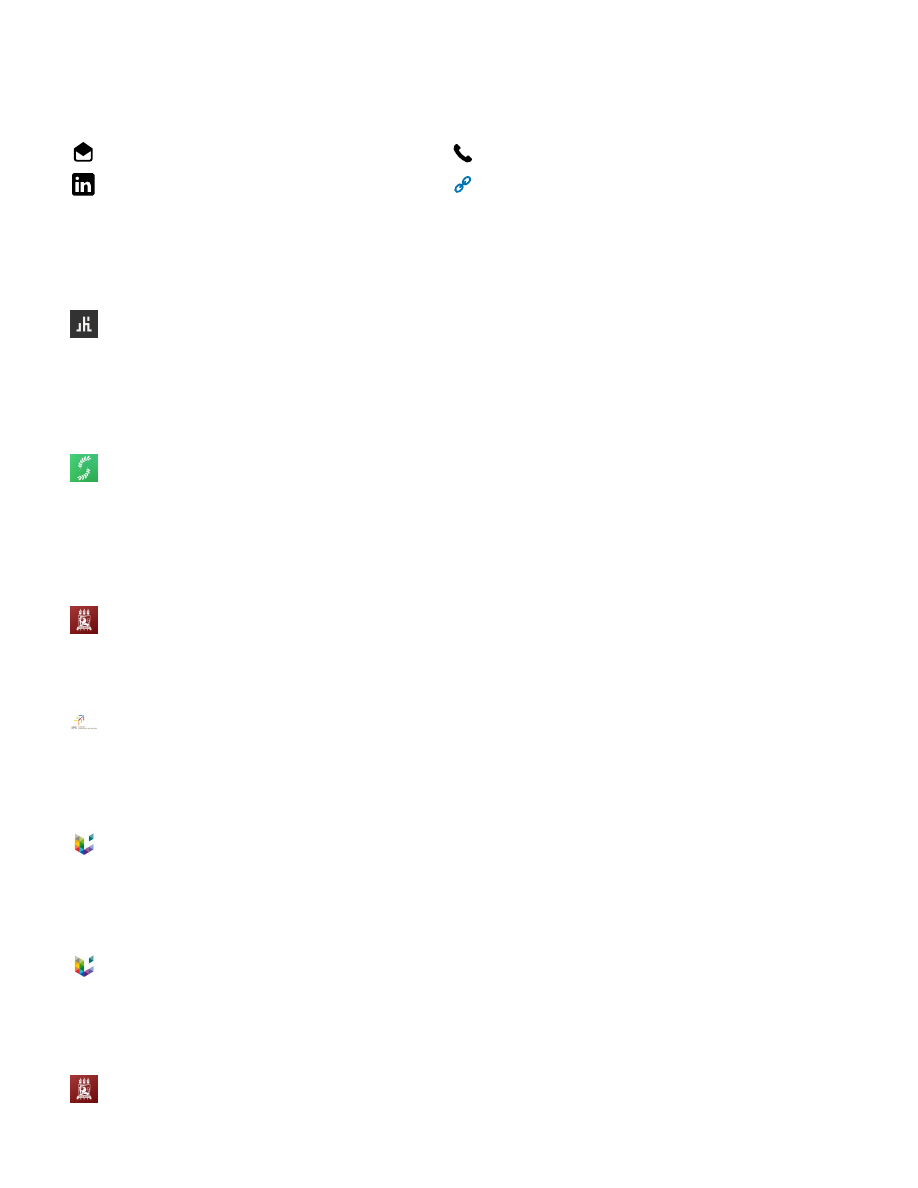
\includegraphics[width=9.5625in,height=12.375in]{Resume-Gabriel-Barros001.png}

Gabriel Barros

gabrieldelc.barros@gmail.com

+5581996007418

\href{https://www.linkedin.com/in/gabriel-del}{linkedin.com/in/gabriel-del}

\url{https://github.com/gabriel-del}

\textbf{Summary}

Full-Stack developer very experienced using linux and Next.js

\textbf{Experience}

\textbf{Software Engineer}

Kindelia Foundation

Apr 2022 - Oct 2022 (7 months)

Front-end developer using Next.js, tailwindcss, turborepo etc.

Functional programer on language Kind.

\textbf{Software Engineer}

Salvus

Aug 2019 - Jan 2020 (6 months)

I developed script to auto calibrate IoT flowmeter using bash, octave,
AWK and C.

\textbf{Education}

\textbf{Universidade Federal de Pernambuco}

Bachelor\textquotesingle s degree, Engenharia Biomédica/Médica

2015 - 2021

\textbf{Polytechnic Institute of Setúbal}

student exchange, Biomedical/Medical Engineering

Sep 2018 - Feb 2019

student exchange

\textbf{University of Liège}

student exchange, Biomedical/Medical Engineering

Sep 2016 - Mar 2017

student exchange

\textbf{University of Liège}

student exchange, French Language and Literature

Oct 2016 - Dec 2016

Cours de français langue étrangère

\textbf{Universidade Federal de Pernambuco}

scientific research, Mathematics

Gabriel Barros - page~1

\hypertarget{page2-div}{}
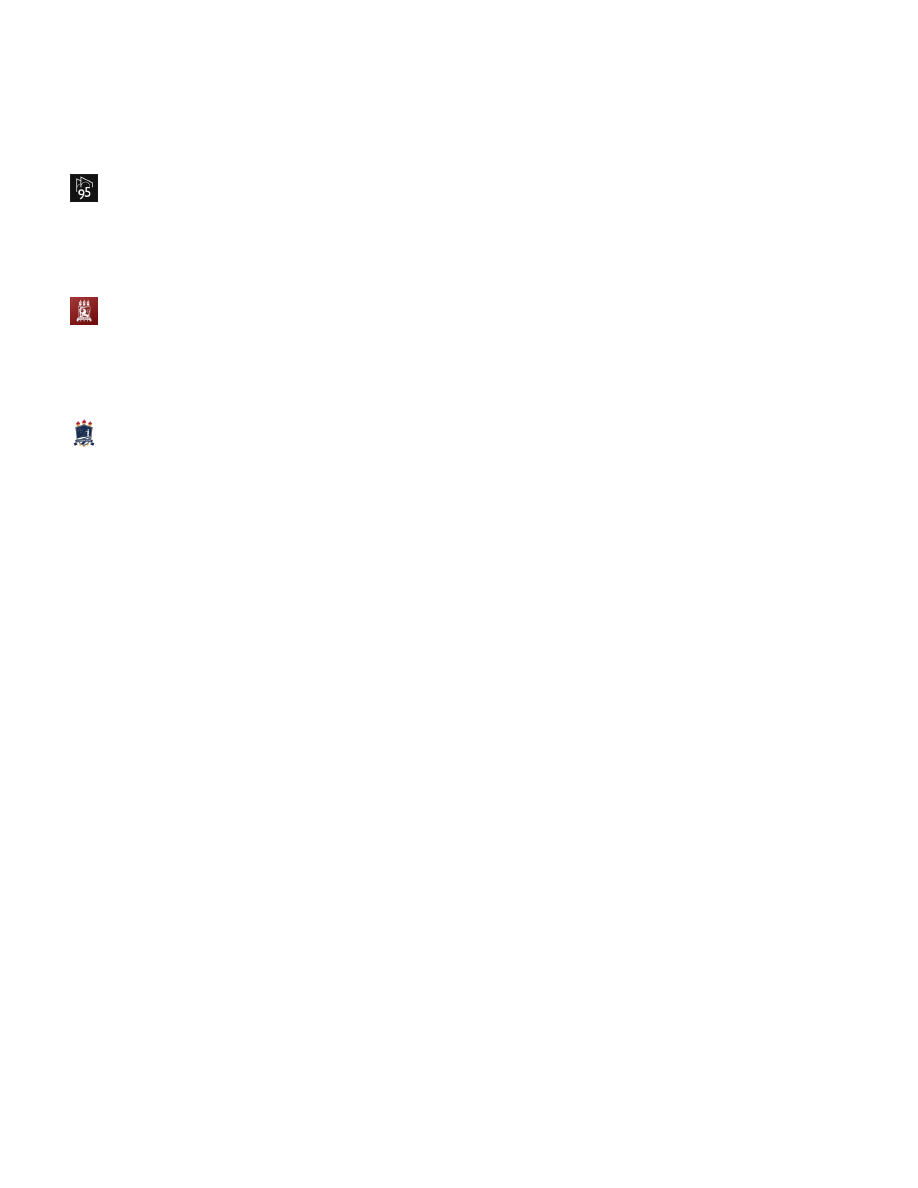
\includegraphics[width=9.5625in,height=12.375in]{Resume-Gabriel-Barros002.png}

Feb 2015 - Jun 2016

scientific research offered by the mathemathics olympics

PICME (Programa de iniciação científica em Matemática)

\textbf{Universidade Federal de Minas Gerais}

Summer course, Mathematics

Jan 2016 - Feb 2016

Course offered by the mathematics olympics

\textbf{Universidade Federal de Pernambuco}

Middle School Diploma, Basic School

Feb 2008 - Dec 2014

Basic School

\textbf{Universidade Federal Rural de Pernambuco}

scientific research, Mathematics

Aug 2009 - Dec 2012

scientific research offered by the mathemathics olympics

PICME (Programa de iniciação científica em Matemática)

\textbf{Skills}

Linux~~ • ~ Next.js~~ • ~ Brazilian Portuguese~~ • ~ Portuguese~~ • ~
Open-Source Software~~ • ~ Higher Education~~ • ~

Data Analysis~~ • ~ Image Processing~~ • ~ Digital Image Processing~~ •
~ Machine Learning

Gabriel Barros - page~2
